\section{Robust Structure From Motion}
\label{sec:sfm}

Given our Gaussian mixture model, we can now detect the similarity between
traces and use this probability to remove traces that decrease the quality of
performing structure from motion.  We first describe the application of our GMM
model to this problem, and then describe the setup and results of our
experiments.

\subsection{Model Application} % (fold)
\label{sub:Model Application}

In structure from motion, we focus on recovering the structure of a
static scene from a mobile camera.  We first note that data
collected from hand-held mobile phones (in our case, a Samsung Galaxy S II)
tends to be much shakier than prior data sets in the literature.  
This has no direct effect on the structure from motion algorithm itself, but we find that 
under these conditions SIFT and KLT are more likely to produce clearly erroneous feature traces,
thereby worsening the end output of structure from motion.  Additionally, we find
that moving objects in the video frame make it difficult for
the structure from motion algorithm to disentangle the motion of the object in
the scene from the motion of the camera, again worsening the results of the
algorithm.  Sighting these two issues, we aim to use or
GMM to improve the results of the structure from motion algorithm.

As explained previously, our GMM detects how similar traces are within a given
scene.  As a result, ``bad traces'' are rated as low probability traces since they 
are shaped quite differently from correct traces, which mostly reflect the motion of 
the camera.  Similarly, moving objects in a scene yield traces very distinct from 
those generated by static objects, also giving them a low probability according to our GMM.  When plotting a
distribution of these traces, as seen in Figure \ref{fig:logpdfs}, we see that
a relatively small portion of the traces have a distinctly lower score than
the rest, which are relatively similar.  We consider this
segment of much lower probability traces to be outliers which should be
removed before performing the structure from motion algorithm.

\begin{figure}[h]
	\begin{subfigure}[b]{0.5\textwidth}
		\centering
		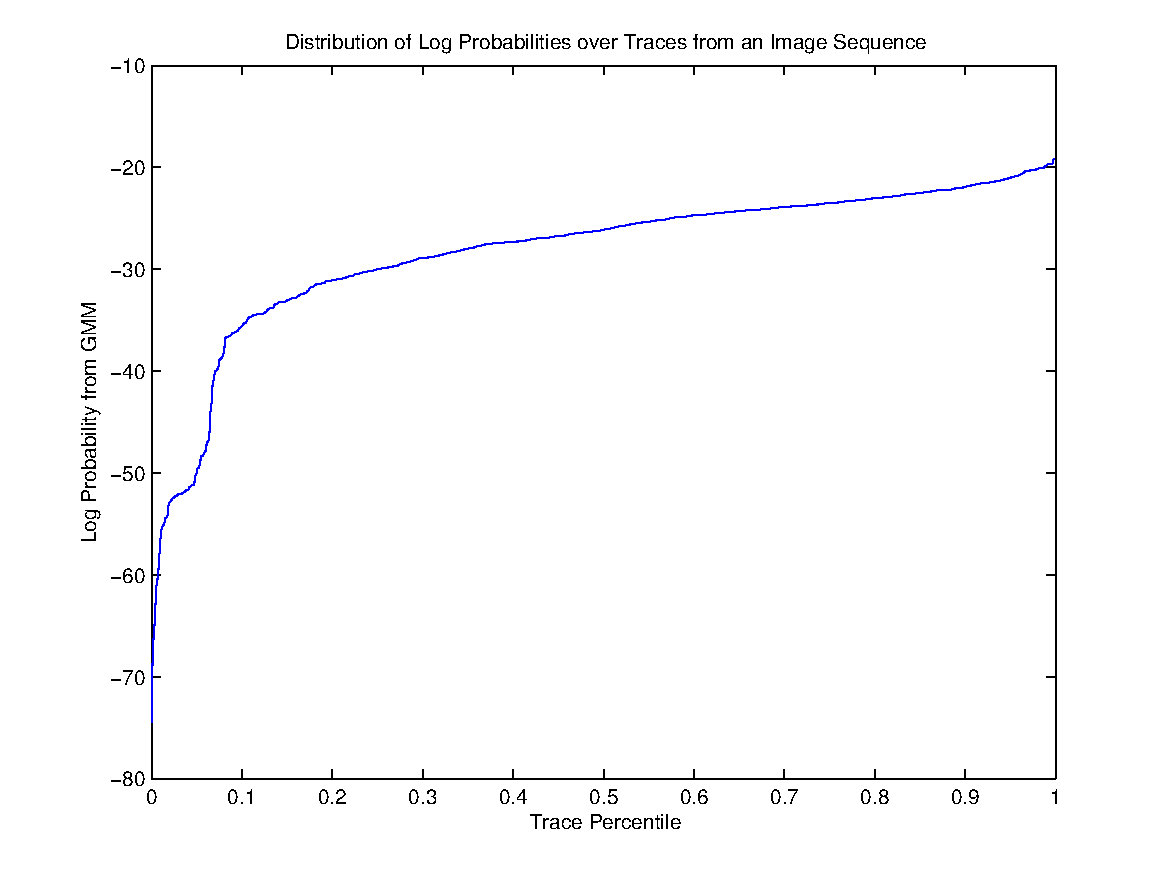
\includegraphics[width=0.9\textwidth]{figs/logpdfs-frame90.pdf}
		\caption{Outdoor dataset}
		\label{fig:logpdfs:90}
	\end{subfigure}%
	\begin{subfigure}[b]{0.5\textwidth}
		\centering
		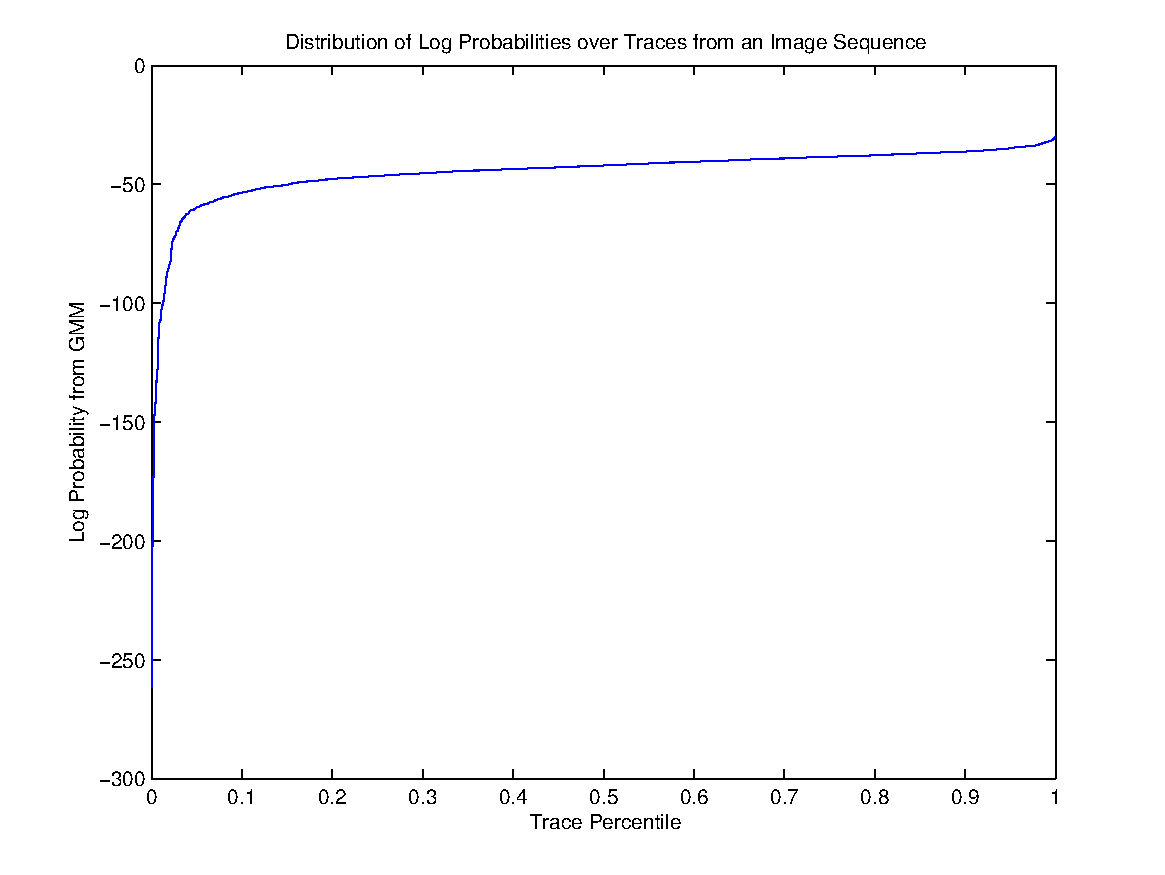
\includegraphics[width=0.9\textwidth]{figs/logpdfs.pdf}
		\caption{Outdoor dataset 2}
		\label{fig:logpdfs:105}
	\end{subfigure}%

	%\begin{center}
		%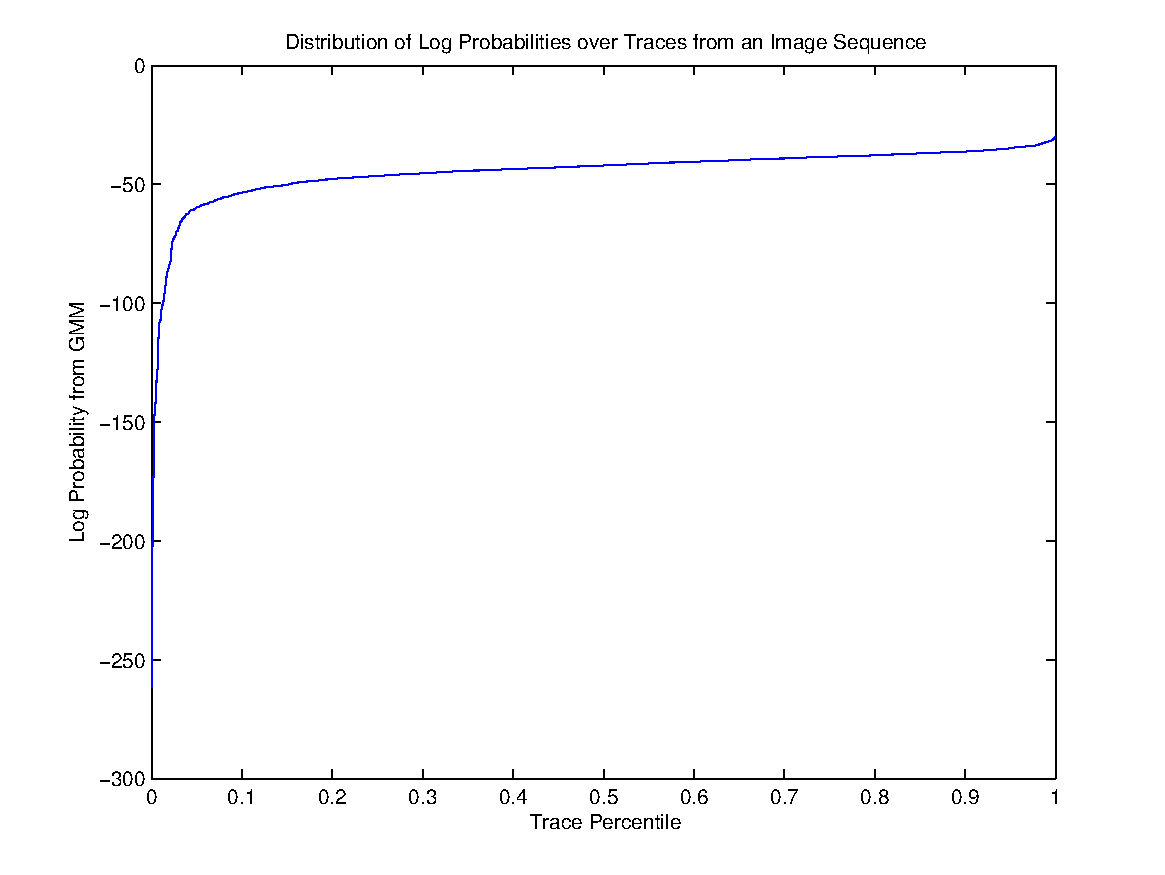
\includegraphics[width=4in]{figs/logpdfs.pdf}
	%\end{center}
	\caption{Distribution of log-probabilities generated by GMM for a set of traces in our ``Outdoor'' datasets}
	\label{fig:logpdfs}
\end{figure}

In our tests we find that using a simple threshold to remove the lowest-scoring 10\% of traces 
is sufficient to cull the most egregious outliers, as the score distributions of most data sets are
similar to that shown in Figure \ref{fig:logpdfs}.  In future work, smart detection of the crtical 
inflection in log probability might produce more desirable results.

% subsection Model Application (end)

\subsection{Experiments} % (fold)
\label{sub:Experiments}

\paragraph{Setup} 
We show the results of our algorithm on short clips from three different scene: 
a desk chair, a lounge chair, and two from outdoors.  For each scene we selected a
continuous sequence of frames from the video so that a large number of points were tracked
across all frames.  For the desk chair we used 30
frames that tracked 164 features; for the lounge chair we used 20 frames that
tracked 508 features; for the outdoor scenes we used 10 frames that tracked
784 features and 15 frames that tracked 1596 features.  In each video we have a substantial
amount of camera motion around a generally static scene.

We evaluate the effectiveness of our GMM filtering operation by comparing the accuracy of the
rank-three approximation before and after the filter.  See Section \ref{sec:background} for
a justification of the rank-three approximation.  We achieve this by comparing the ratio of the largest singular value
of the data matrix $D$ to the sum of the fourth-and-up singular values.  We call this the ``Purity Score'' of the data: 
\begin{align}
	D = U\Sigma V\tr \\
	{\rm Purity\ Score} &= \frac{\sigma_1}{\sum_{i > 3} \sigma_i}.
\end{align}
Because all $\sigma_i$ in the denominator should be small, the larger the
purity score, the more clean the data in $W$ is and the better the result of
structure from motion.

\paragraph{Results} 

To visually evaluate the effectiveness of our method, we overlay features traces 
from a scene, color coded by GMM score, onto the first frame of the video, as shown
 in Figure \ref{fig:colored-traces}.  Traces with
higher probability are colored green, and traces with lower probability (outliers) are
colored red. 

In Figure \ref{fig:colored-traces}(a) and (b) we see that feature tracking
algorithm occasionally finds faulty traces when trying to track a feature along
the carpet.  In each case we see that the shape of the trace is largely
different than that of other traces in the scene.  In Figure
\ref{fig:colored-traces}(c), the algorithm notices that a man walked through
the middle of the scene while filming it.  As a result, his traces show his
motion as well as the camera motion and are largely different than the traces
from the static objects in the scene.  Our algorithm successfully detects this
and gives these traces a low probability through the GMM.

\begin{figure}[tb]
	\hspace{-0.6cm}
	\begin{minipage}[b]{0.5\linewidth}
		\centering
		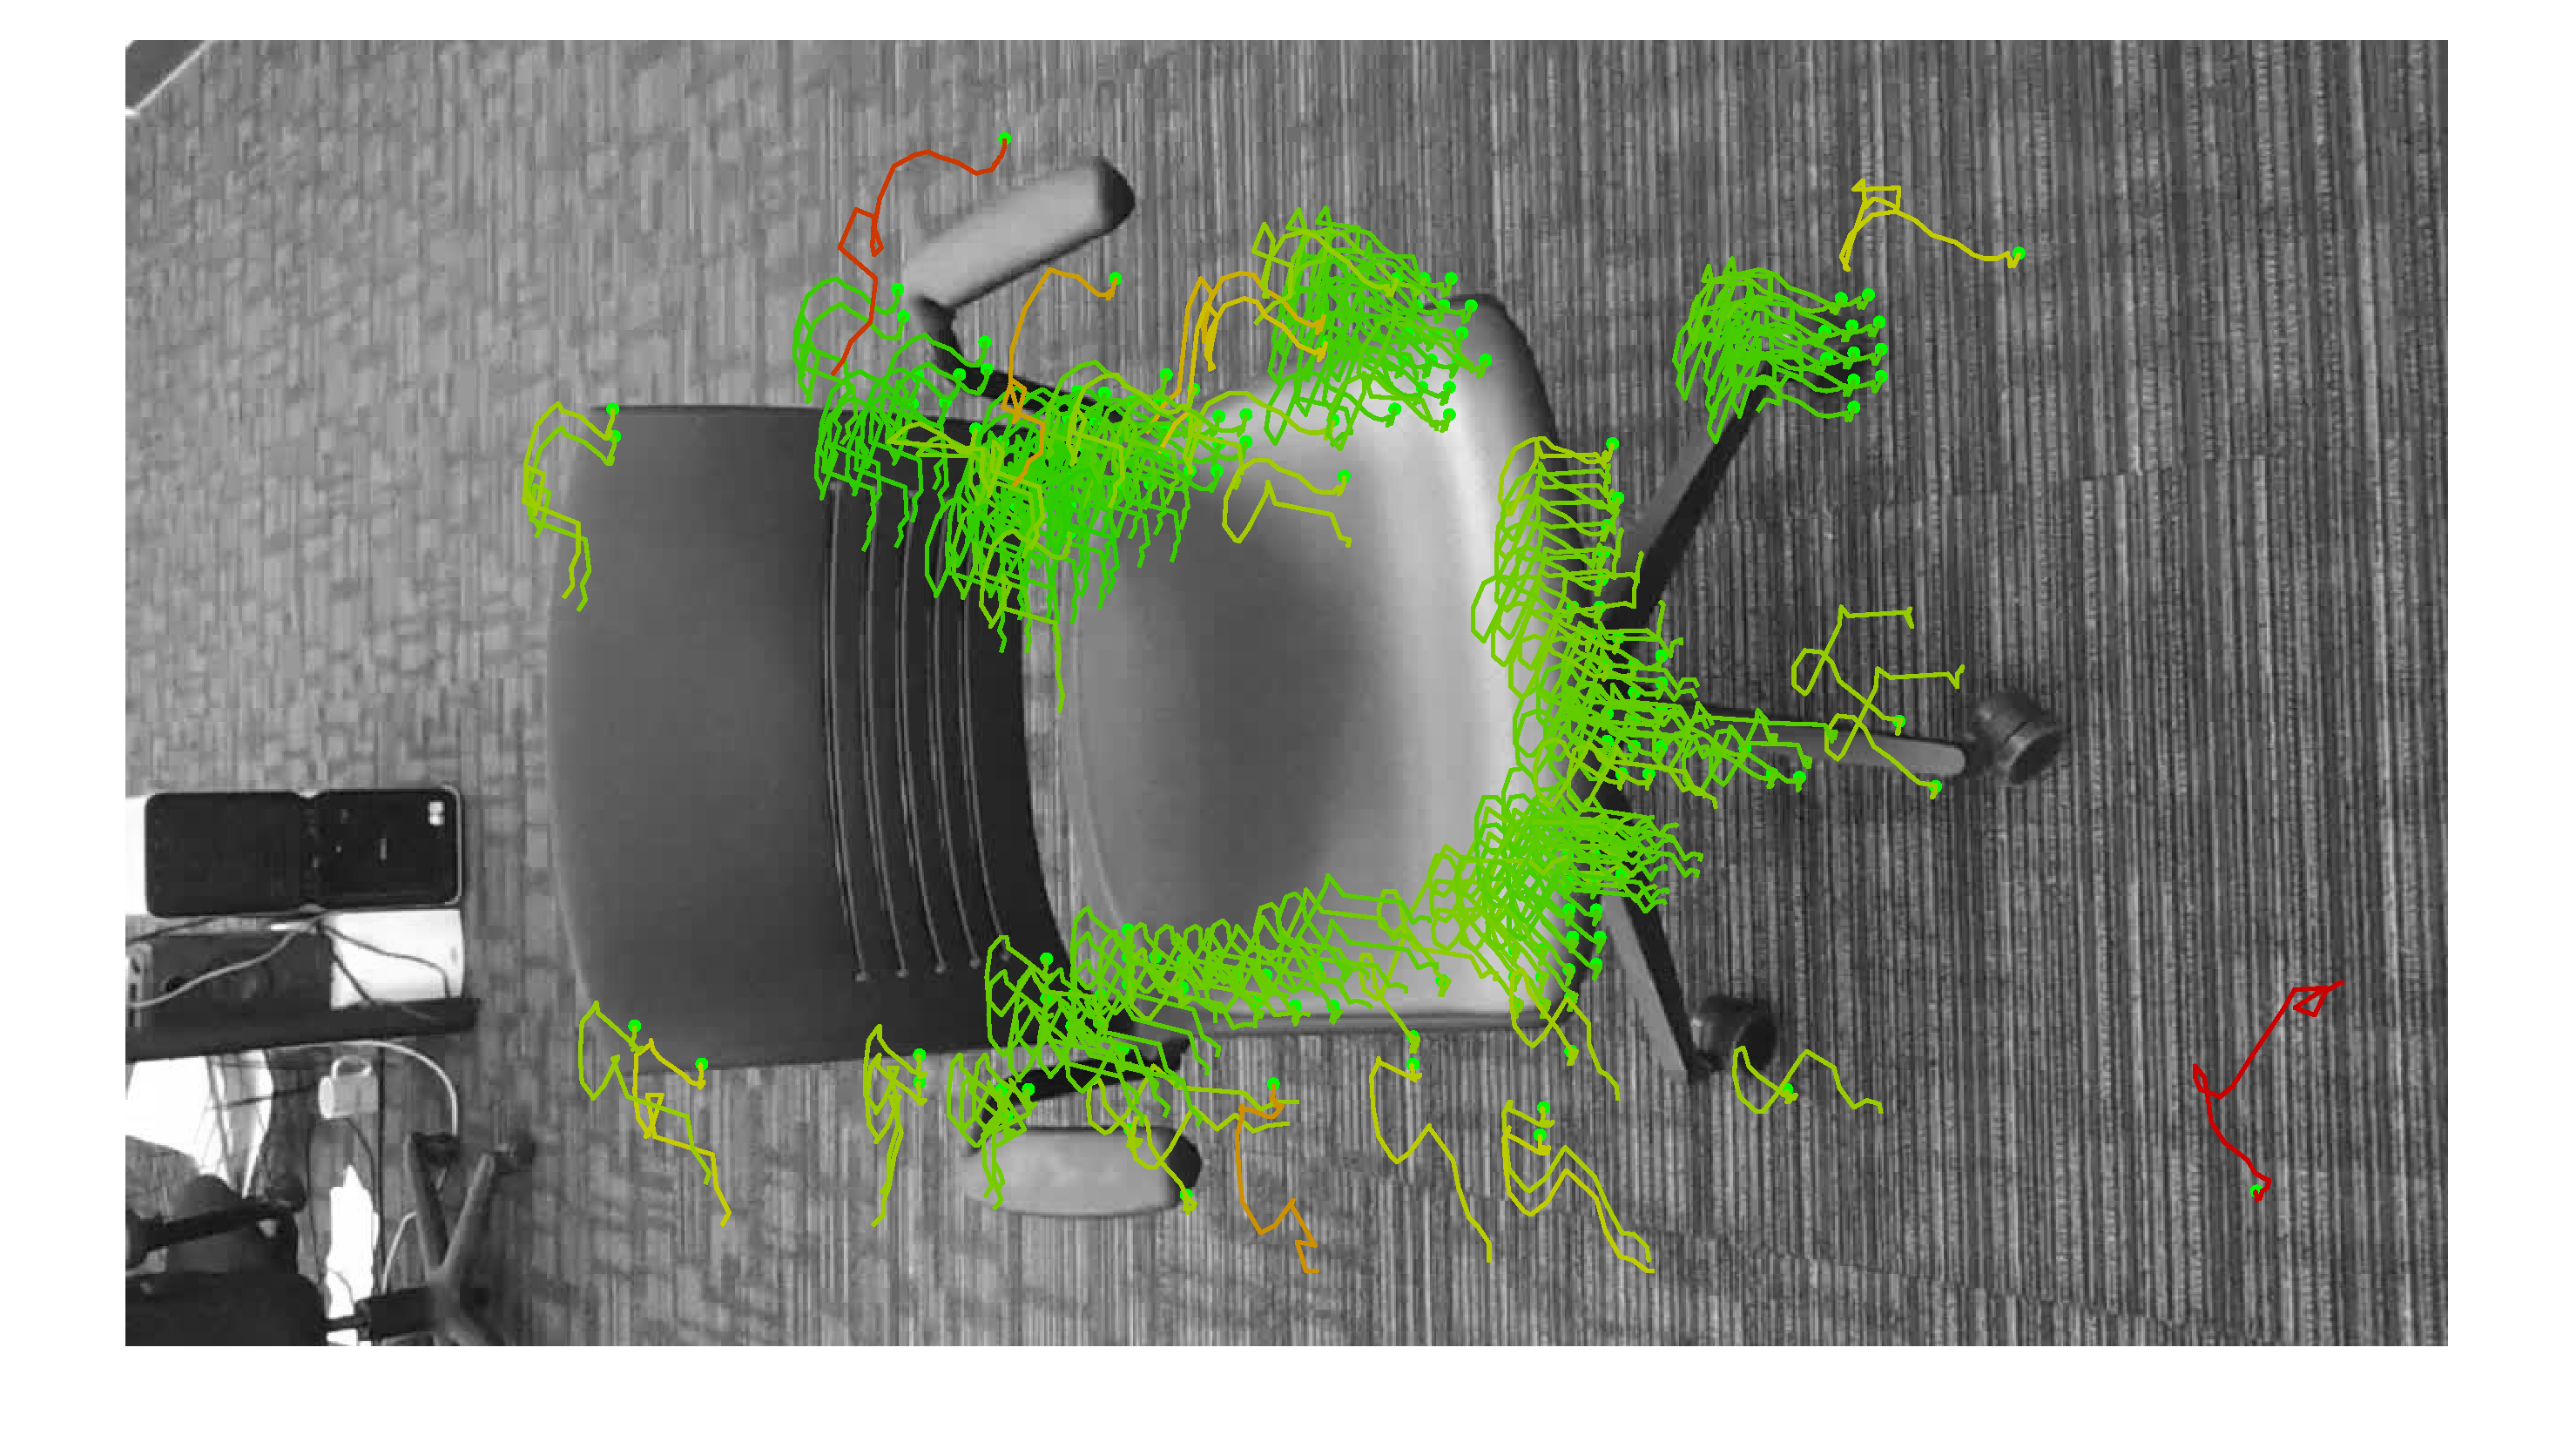
\includegraphics[height=2.1in,angle=-90]{figs/desk-1.pdf}\\ (a)
		%\caption{default}
	\end{minipage}
	\hspace{0cm}
	\begin{minipage}[b]{0.5\linewidth}
		\centering
		\begin{minipage}[b]{\linewidth}
			\centering
			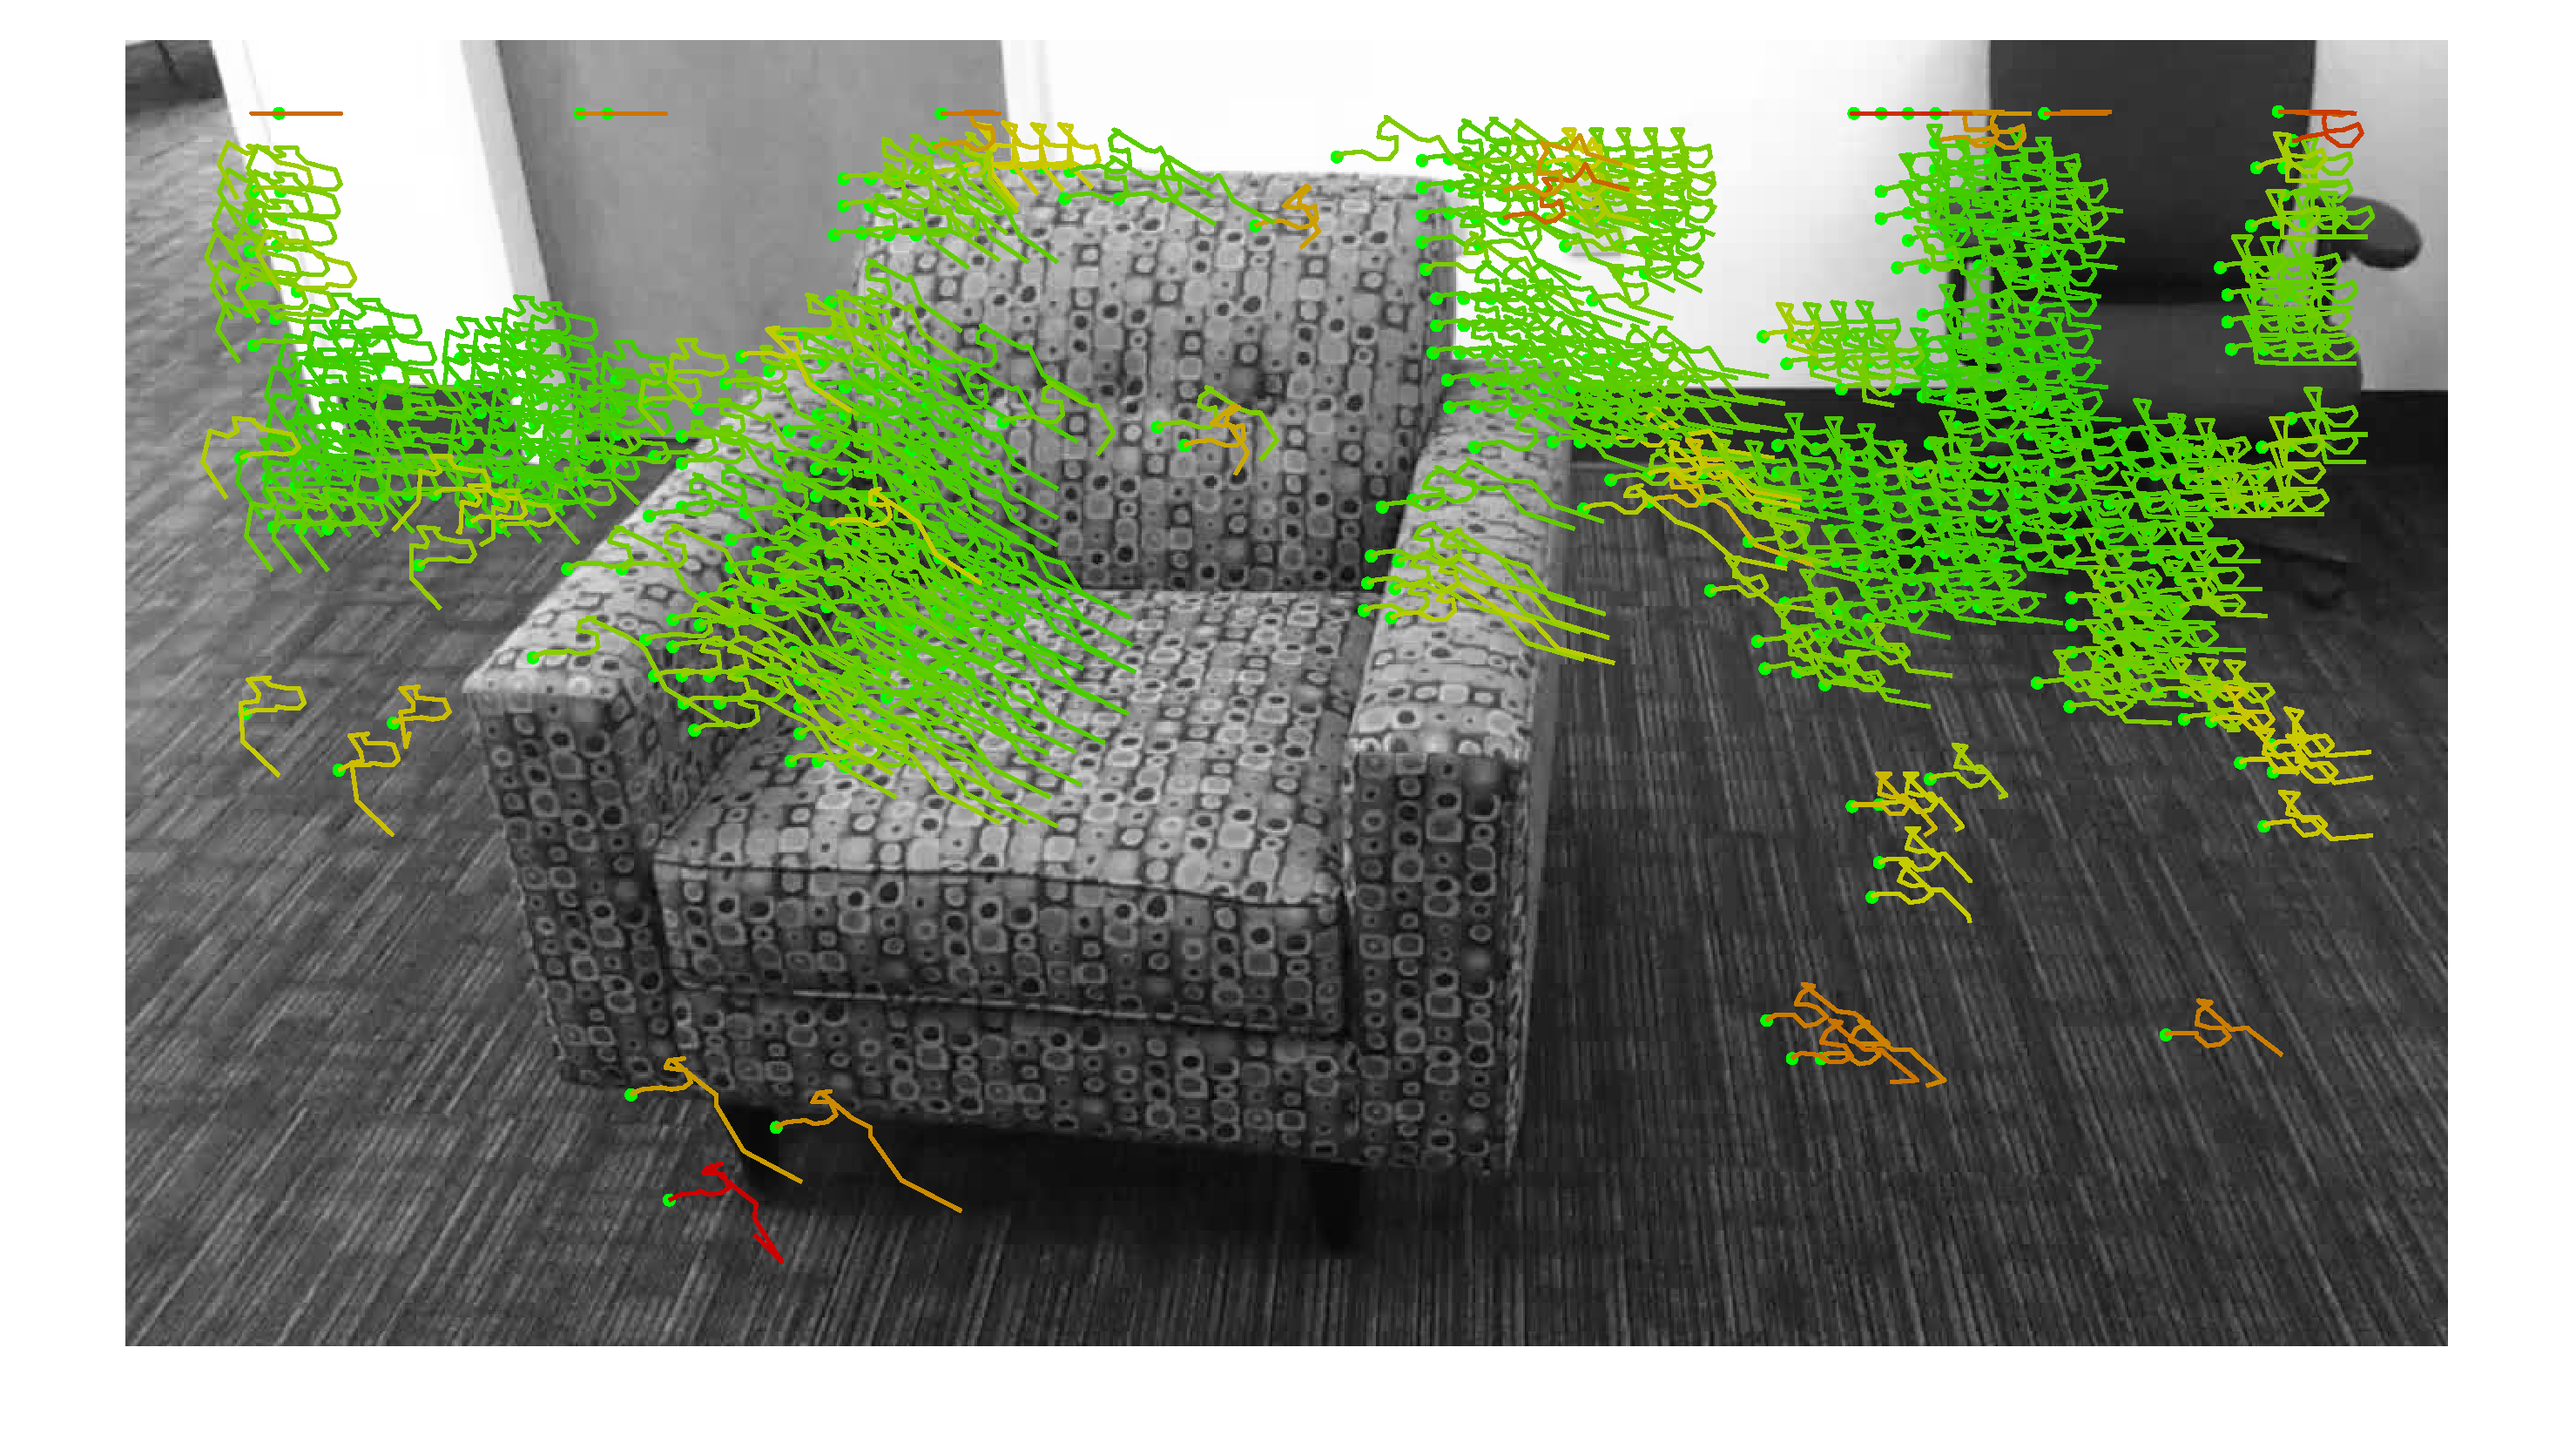
\includegraphics[width=3in]{figs/lounge-1.pdf} \\ (b)
			%\caption{default}
		\end{minipage}
		\vspace{0.1cm}
		\begin{minipage}[b]{\linewidth}
			\centering
			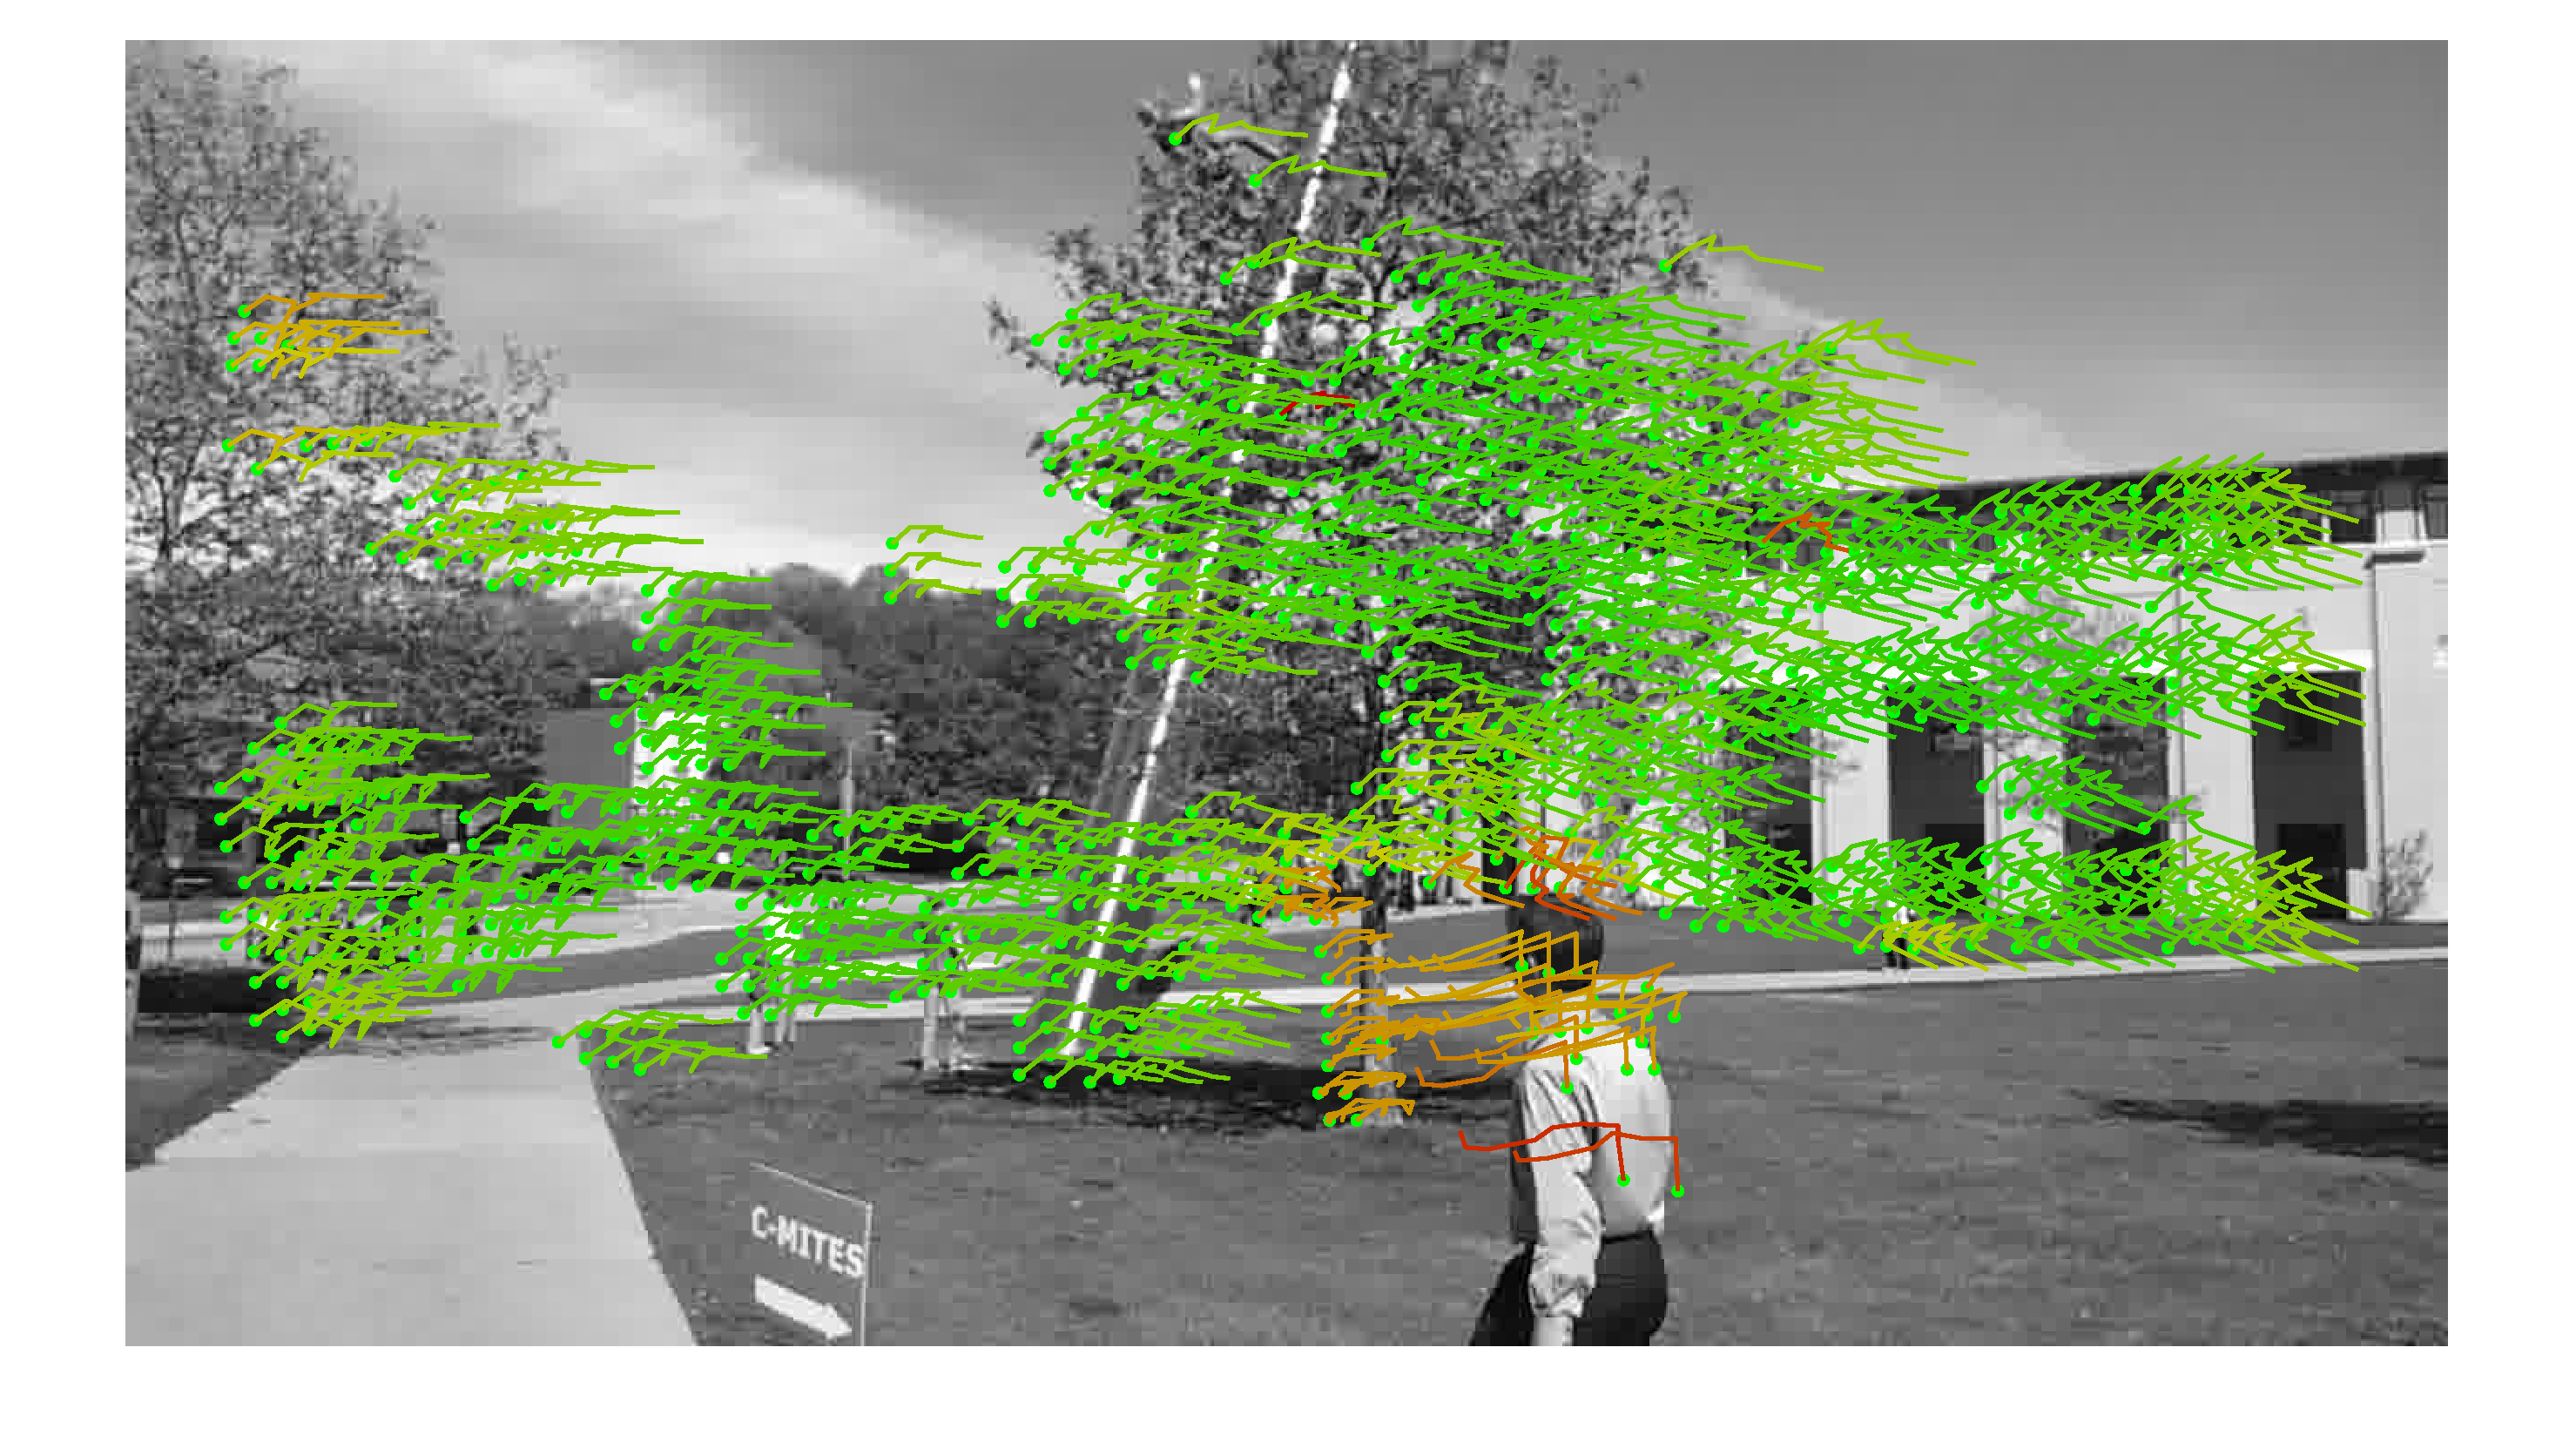
\includegraphics[width=3in]{figs/outdoor3-90.pdf} \\ (c)
			%\caption{default}
		\end{minipage}

	\end{minipage}
	\caption{Traces colored by GMM score for (a) desk chair, (b) lounge chair, and (c) outdoors.  Green reflects a high GMM score and red reflects a low GMM score.}
	\label{fig:colored-traces}
\end{figure}


In addition to visually evaluating the success of our algorithm in isolating
outlier traces, we compared the purity score of the data before and after
outlier removal.  In running our algorithm and evaluation across all four data
sets, we found that in every case outlier removal improved the purity score and
thus structure from motion result.  The purity score comparison can be seen in
Table \ref{tab:purities}.  Not surprisingly, the algorithm seems to be most
useful when there is a moving object in the scene, as this results in a large
number of outlier points that would disrupt the structure from motion
algorithm.  Overall, we considered our method to work as intended and improved
the resulting structure from motion.

\begin{table}[tb]
	\begin{center}
		\begin{tabular}{|l|c|c|}
			\hline
			\multirow{2}{*}{Data Set}  &\multicolumn{2}{|c|}{Purity Score}\\ \cline{2-3}
			& \multicolumn{1}{|c|}{Original}  & \multicolumn{1}{|c|}{With Outlier Removal}\\ \hline
			Desk Chair & 36.14 & 40.63 \\ \hline
			Lounge Chair & 89.2 & 111.36 \\ \hline
			Outdoors & 90.43 & 175.44 \\ \hline
			Outdoors 2 & 96.37 & 127.96 \\ \hline
		\end{tabular}
	\end{center}
	\caption{Comparison of Purity Score before and after outlier removal.}
	\label{tab:purities}
\end{table}


% subsection Experiments (end)
